\section{Models of Indentation in Atomic Force Microscopy \label{Appendix: Models of Indentation in Atomic Force Microscopy}}
\subsection{Hertz Model \label{Appendix: Hertz}}

The Hertz model is the most prevalent model used for AFM indention and describes contact forces for isotropic and homogeneous materials, denoted as elastic half-spaces, which present a linearly elastic response to forces\cite{kontomaris2019determination} and are assumed to extend infinitely in all directions with a flat boundary on the top surface.\cite{kontomaris2019harmonic}. This necessitates the AFM tip radius be at least ten times smaller than the sample dimension for the assumption to hold. In addition, it is assumed that the contract is smooth and continuous with no friction or adhesion\cite{kontomaris2019determination}.  

\begin{figure}[H]
    \centering
    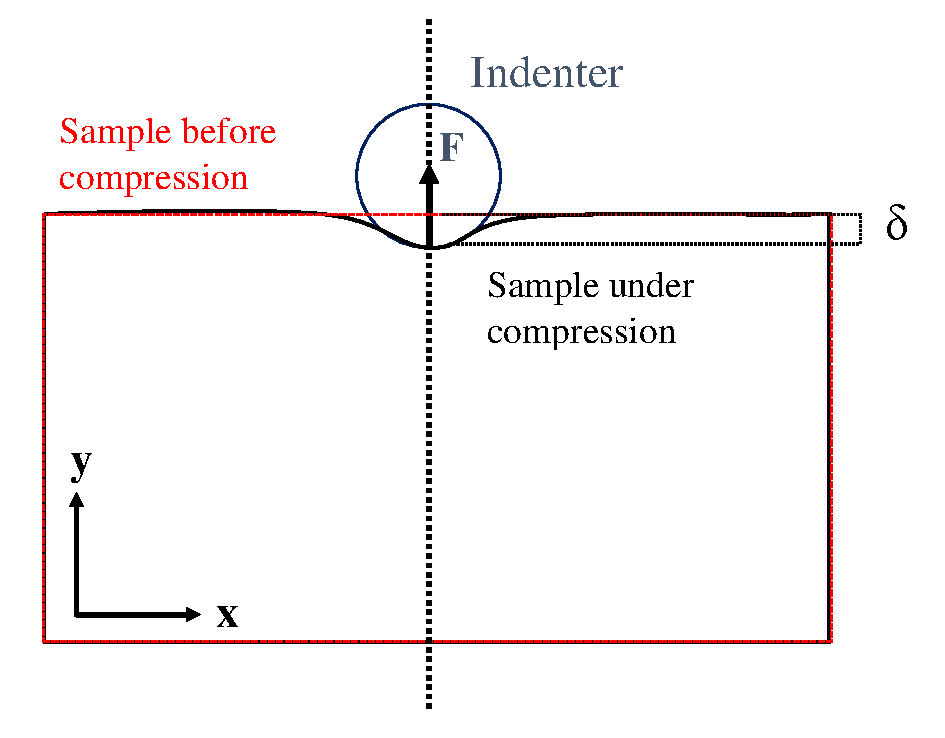
\includegraphics[width=0.6\linewidth]{Figures/Hertz Contact.pdf}
    \caption{\label{fig: Hertz Contact} Illustration of contact experienced by elastic half-space.  Where $\delta$ is indentation depth of the indenter into surface, $F$ is total force of indentation.}
    
\end{figure}


Subsequently, the Hertz model provides the relation between the applied force, F, and the indentation depth, $\delta$, \cite{kontomaris2018hertz,kontomaris2020hertz}

\begin{equation} F_{Hertz}(\delta) =  \frac{4}{3} \frac{E_2}{(1-\nu_2^2)} \sqrt{R_{12}} \delta^{3/2} \label{eq: Hertz} \end{equation}

$$\frac{1}{R_{12}} = \frac{1}{R_{1}} + \frac{1}{R_{2}} $$

where $R_{12}$ is the tip-surface contact radius, $R_1$ is indenter radius, $R_2$ is surface radius ($\inf$ for a plane) $E_2$ Young’s modulus and $\nu_2$ is the Poisson’s ratio of the sample. This relation allows calculation of Young’s modulus as a fitting parameter for experimental measurements of force curves \cite{dokukin2013quantitative,vinckier1998measuring,glaubitz2014novel}. In addition, taking the logarithm of this equation returns a linear equation:

\begin{equation} \log\left(F_{Hertz}(\delta) \right) = \frac{3}{2}\log(\delta) + \log\left(\frac{4}{3} \frac{E_2}{(1-\nu_2^2)} \sqrt{R_{12}}\right) \label{eq: Hertz Log}\end{equation}

Subsequently, this equation can be used to cast indentation data in dimensional units of for force ($\frac{F}{E^*R^2}$) and indentation ($\delta/R$), such that:

\begin{equation} \frac{F_{Hertz}(\delta)}{E^*R_{12}^2}  =  \frac{4}{3}(\frac{\delta}{R_{12}})^{3/2} \label{eq: Hertz Dimensionless} \end{equation}

\begin{equation} F_{Dimensionless}  =  \frac{4}{3}(\delta_{Dimensionless})^{3/2} \label{eq: Dimensionless Units} \end{equation}

where $E^* = \frac{E_2}{(1-\nu_2^2)}$. Therefore, $F_{Dimensionless} = \frac{F_{Hertz}}{E^*R_{12}^2}$ and $\delta_{Dimensionless} = \frac{\delta}{R_{12}}$. 

\subsection{Other Hertzian Model}
The Hertz model ignores adhesive and frictional forces and can only be applied for parabolic tips (and approximately for a spherical tip given that $h \ll R$). However, various other 'Hertzian' contact models\cite{korayem2014modeling}, including the models of Sneddon\cite{harding1945elastic,han2021modified}, JKR\cite{johnson1971surface} , DMT\cite{derjaguin1975effect}, BCP\cite{burnham2020surface}, COS\cite{carpick1999general}, PT\cite{pietrement2000general}, and SUN\cite{sun2004using}, use the same base dynamics but incorporate various other adhesive forces, tip geometry and dynamics, and constraints to obtain more advanced models of contact mechanics. Some other models used are discussed below.


\subsection{Dimitriadis Model\label{Appendix: Dimitriadis}}
A more complex model that is applied to spherical indenters for soft materials in AFM experiment is the model by Dimitriadis \textit{et al} \cite{DIMITRIADIS20022798}.

\begin{equation} 
\begin{split}
F_{Dimitriadis}(\delta) = & \frac{4}{3}\frac{E_{2}}{(1-\nu_{2}^2)}R_{12}^{1/2}\delta^{3/2} \left[ 1 - \frac{2\alpha_0}{\pi}\chi + \left(\frac{2\alpha_0}{\pi}\chi\right)^2 \right. \\ 
& -\left. \left(\frac{2\alpha_0}{\pi}\chi\right)^3 +  \left(\frac{2\alpha_0}{\pi}\chi\right)^4 -\frac{16}{\pi^2}\beta_0 \left( \frac{2\pi}{15}  - \frac{3}{5}\alpha_0\chi \right)\chi^3 \right]
\end{split} 
\label{eq: Dimitriadis}
\end{equation}

where $R_{12}$ is the radius of contact between the tip and the surface $\frac{1}{R_{12}} = \frac{1}{R_{1}} + \frac{1}{R_{2}} $, $R_1$ is the indenter radius, $R_2$ is the surface radius ($\inf$ for a plane) Young's modulus $E_2$ and $\nu_2$ is the Poisson’s ratio of the sample. And 

$$\chi = \frac{\sqrt{R_{12}\delta}}{h}$$
$$\alpha_0 = -0.347\frac{3-2\nu_{2}}{1-\nu_{2}}$$
$$\beta_0 = 0.056\frac{5-2\nu_{2}}{1-\nu_{2}}$$


\subsection{Sneddon Model\label{Appendix: Sneddon}}

Applying the Hertz model to conical indenters, we recover the Sneddon model\cite{han2021modified} given as

\begin{equation}F_{Sneddon}(\delta) = \frac{2}{\pi}\frac{E_2}{(1-\nu_2^2)}tan(\alpha)\delta^{2}\label{eq: Sneddon}\end{equation}

where $\alpha$ is indenter principle angle, $R_2$ is surface radius ($\inf$ for a plane) $E_2$ Young’s modulus and $\nu_2$ is the Poisson’s ratio of the sample.  In addition, taking the logarithm of this equation returns a linear equation: 

\begin{equation} \log\left(F_{Sneddon}(\delta) \right) = 2\log(\delta) + \log\left(\frac{2}{\pi}\frac{E_2}{(1-\nu_2^2)}tan(\alpha)\right) \label{eq: Sneddon Log} \end{equation}

\subsection{Double Contact Model\label{Appendix: Double Contact}}

Indentation into elastic spheres presents a more complex analysis as we must account for both the indentation between the indenter and the surface and the indentation between the surface and the base. As seen in Figure \ref{fig: Double Contact}, part of the indenter of the displacement is due to the compression of the elastic sphere into the base $\delta^*_{32}$. Moreover, the reaction force between the indenter and sphere will be enhanced as the indenter creates reaction force both due to its indentation into the sample and due to the compression of the sample between the indenter and base. To account for this, we consider double contact models\cite{dokukin2013quantitative,glaubitz2014novel}. 

\begin{figure}[H]
    \centering
    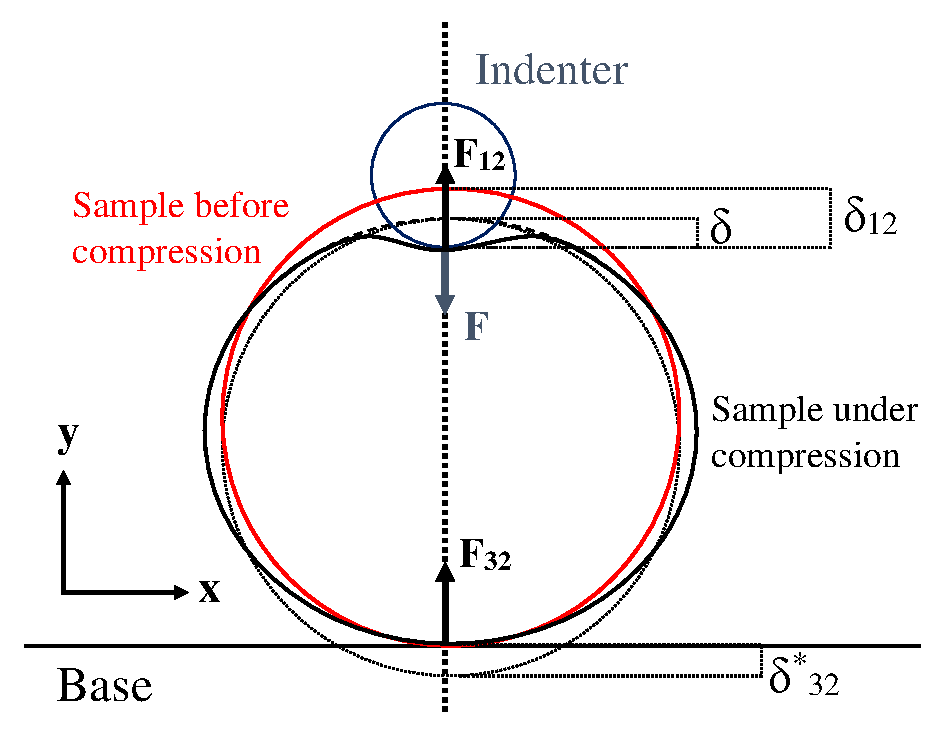
\includegraphics[width=0.6\linewidth]{Figures/Double Contact.pdf}
    \caption{\label{fig: Double Contact} Illustration of double contact experienced by spherical sample.  Where $\delta$ is indentation depth of the indenter into surface, $\delta_{12}$ is total displacement of the indenter, $\delta^*_{32}$ indentation depth of the surface into base, $F$ is total force of indentation, $F_{12}$ is contact force experienced by indenter, $F_{32}$ contact force experienced by base. In these models, the corrected values for indentation depth are calculated by subtracting the displacement/ compression of the surface at its base from the displacement of the indenter. For the corrected force, we sum the reaction force between the indenter and surface and the force between the base and surface. This is as the force due to the indenter will be distributed between both the reaction at the base and the indenter. }
\end{figure}

In these models, the corrected values for indentation depth are calculated by subtracting the displacement/ compression of the surface at its base from the displacement of the indenter. 

\begin{equation}\delta = \delta_{12}-\delta^*_{32}\label{eq: Corrected Indentation}\end{equation}

where $\delta$ indentation depth of the indenter into surface, $\delta_{12}$ is indentation displacement of the indenter, $\delta^*_{32}$ indentation depth of the surface into base. For the corrected force, we sum the reaction force between the indenter and surface and the force between the base and surface. This is as the force due to the indenter will be distributed between both the reaction at the base and the indenter.

\begin{equation} F = F_{12}+F_{32}\label{eq: Corrected Force}\end{equation}

where $F$ is total force of indentation, $F_{12}$ is contact force experienced by indenter, $F_{32}$ contact force experienced by base.


\subsection{Hertz Double Contact\label{Appendix: Hertz Double}} 
 Surface - Spherical Indenter Indentation (Hertz)
 
\begin{equation} \delta_{12}(F) = \left( \frac{3}{4} \frac{(1-\nu_2^2)}{E_2} \frac{F}{\sqrt{R_{12}}} \right)^{2/3}\end{equation}

 Spherical Surface 
$$ \frac{1}{R_{12}} = \frac{1}{R_{1}} + \frac{1}{R_{2}} $$

 Flat Surface 
$$R_{32} = R_{2}$$

 Calculating Double Contact

$$ \delta_{12}(F) = \delta(F) + \delta_{32}^*(F)  $$

$$ =    \left( \frac{3}{4} \frac{(1-\nu_2^2)}{E_2} \frac{F}{\sqrt{R_{12}}} \right)^{2/3}  +     \left( \frac{3}{4} \frac{(1-\nu_2^2)}{E_2} \frac{F}{\sqrt{R_{32}}} \right)^{2/3}
$$

$$ =    \left( \frac{3}{4} \frac{(1-\nu_2^2)}{E_2} \cdot F \right)^{2/3} \left[ \frac{1}{R_{12}^{1/3}}  + \frac{1}{R_{32}^{1/3}} \right] 
$$

$$ =    \left( \frac{3}{4} \frac{(1-\nu_2^2)}{E_2} \cdot F \right)^{2/3} \left[ \frac{R_{12}^{1/3}+R_{32}^{1/3}}{(R_{12}R_{32})^{1/3}} \right] 
$$

\begin{equation}  F(\delta_{12}) =  \frac{4}{3} \frac{E_2}{(1-\nu_2^2)} \left[ \frac{(R_{12}R_{32})^{1/3}}{R_{12}^{1/3}+R_{32}^{1/3}} \right]^{3/2}\delta_{12}^{3/2} \label{eq: Hertz Double Contact}\end{equation}

where $\delta$ indentation depth of the indenter into surface, $\delta_{12}$ is indentation displacement of the indenter, $\delta^*_{32}$ indentation depth of the surface into base and $F$ is contact force experienced by indenter. $R_{12}$ is the tip-surface contact radius, $R_{32}$ is the surface-base contact radius, $R_1$ is indenter radius, and $R_2$is surface radius. $E_2$ Young’s modulus and $\nu_2$ is the Poisson’s ratio of the sample.

\subsection{Hertz-Sneddon Double Contact \label{Appendix: Sneddon Double}}
Using a similar methodology for Sneddon and Hertz we formulate our own double contact model for conical indenters: 

Model for Surface - indenter (Sneddon)
$$ \delta_{12}(F) = \left(\frac{\pi}{2}\frac{(1-\nu_2^2)}{E_2} \frac{F}{tan(\alpha)}\right)^{1/2}$$

 Model for Surface-Base Indention (Hertz)
$$ \delta_{32}(F) = \left( \frac{3}{4} \frac{(1-\nu_2^2)}{E_2} \frac{F}{\sqrt{R_{32}}} \right)^{2/3}$$

 Flat Surface 
$$R_{32} = R_{2}$$

 Calculating Double Contact

$$ \delta(F) = \delta_{12}(F) + \delta_{32}^*(F)  $$

$$ = \left(\frac{\pi}{2}\frac{(1-\nu_2^2)}{E_2} \frac{F}{tan(\alpha)}\right)^{1/2}  +  \left( \frac{3}{4} \frac{(1-\nu_2^2)}{E_2} \frac{F}{\sqrt{R_{32}}} \right)^{2/3}
$$

Let the conical term dominate, and for the spherical term  $2/3 \approx 1/2$

\begin{equation} =  \left( \frac{3}{4} \frac{(1-\nu_2^2)}{E_2} F \right)^{1/2} \left(\frac{1}{R_{32}}^{1/4} + (\frac{2\pi}{3}\frac{1}{tan(\alpha)})^{1/2} \right)   \end{equation}

\begin{equation}  F(\delta_{12}) =  \frac{4}{3} \frac{E_2}{(1-\nu_2^2)} \left[ \frac{1}{\left(\frac{1}{R_{32}}^{1/4} + (\frac{2\pi}{3}\frac{1}{tan(\alpha)})^{1/2} \right)} \right]^{2}\delta_{12}^{2}\label{eq: Sneddon Double Contact} \end{equation} 

where $\delta$ indentation depth of the indenter into surface, $\delta_{12}$ is indentation displacement of the indenter, $\delta^*_{32}$ indentation depth of the surface into base and $F$ is contact force experienced by indenter. $R_{12}$ is the tip-surface contact radius, $R_{32}$ is the surface-base contact radius, $R_1$ is indenter radius, and $R_2$is surface radius. $E_2$ Young’s modulus and $\nu_2$ is the Poisson’s ratio of the sample.
